\documentclass[./thesis.tex]{subfiles}

 
\begin{document}

\section{def}

\section{PT2 vs CIPSI}

CIPSI and PT2, all approximations aside, both imply computation of all $\epsilon(\alpha)$, so both can be computed at the same time. CIPSI is about identifying the set of the largest ones, PT2 is about computing the sum over all of them. There are two main consequences to this
\paragraph{PT2 is one iteration behind CIPSI}
In a practical sense, CIPSI is ahead of PT2. A iteration $n$, identifiying the most significant $\ket \alpha$ is about building $\Psi^{n+1}$ while summing them is about estimating the cost of truncation for $\Psi^{n}$. Computing PT2 for a "final" wavefunction therefore requiers an extra iteration, which applies to a larger $\Psi$ and thus is more costly. ( autres implementation de PT2 possible ).

\paragraph{CIPSI can take more approximations}
Fully computing the sum has to be more costly than just identifying the greatest terms. As was said in SELECTION, the CIPSI algorithm can take pretty drastic approximations%, because we only try to identify the set of $\ket \alpha$ with the largest contributions $\epsilon(\alpha)$.
	\begin{itemize}
		\item{$t_g$}
		allows to explore a reduced subset of $\ket \alpha$ in which we are almost sure to find those of interest.
		\item{$t_s$}
		allows for a less accurate and less expensive computation of $\epsilon(\alpha)$, which is unlikely to significantly change the identified set.
	\end{itemize}
	These approximations do not apply when computing PT2. The very large number of smaller contributions makes them much harder to neglect. Unfortunately, increasing $t_g$ and $t_s$ thresholds dramatically increases the computational cost.


\paragraph{}

Unfortunately, a partial computation of PT2 results in a biased value. Since $\epsilon(\alpha)$ is an energy contribution, it's necessarily negative, and PT2 is a sum of same-sign contributions. Therefore, truncating it inevitably results in a bias, some energy is missing but there is little clue how much exactly. The $t_g$ and $t_s$ thresholds used in CIPSI can be seen as ways of minimizing this truncation's amplitude for a given computational cost.

Before the stochastic computation of PT2 was set up, our best choice was to set low thresholds for $t_g$ and $t_s$ while performing CIPSI and accept very approximated values for PT2 of intermediary wavefunctions ; then, once the selection was completed, we would highen them just for a final, very costly ``PT2 only'' iteration. In fact, an exact computation with $t_g=N_{gen}$ and $t_s=N_{det}$ was often prohibitively long, so the final PT2 was still biased. 


We eventually solved this problem by turning the bias into an error bar. The base idea is that, instead of trying to get the largest possible chunk of contribution, we can randomly pick $\epsilon(\alpha)$ contributions and make a Monte-Carlo estimate for the sum over all $\ket \alpha$. In this case, to avoid any bias we must set

$$t_g = N_{gen} ; t_s = N_{det}$$

Not only the estimate will be unbiased and much closer to the actual PT2, but we will have an estimate for the error. Because PT2 is itself used as an approximation

$$E_{var} + E_{PT2} \simeq E_{fullCI}$$

An error significantly smaller than the typical accuracy of $E_{var} + E_{PT2}$ VS $E_{fullCI}$ is certainly acceptable.


For different reasons, the actual Monte-Carlo computation is significantly more convoluted than simply drawing random $\ket \alpha$.


\section{The sample space}


\paragraph{Initial note : ``Sample'' and ``Comb''}
Because of its original nature, this algorithm casts some ambiguity on what should be refered to as a ``sample''. We are going to estimate a sum of elementary contributions $E(I)$, compute and store them individually, and draw them based on a repartition function ; therefore they will be refered to as the \emph{samples}. But the values actually treated as samples in the statistical sense, are sums over several $E(I)$, refered to as \emph{combs}.




\paragraph{$\epsilon(\alpha)$ are packed into elementary contributions $E(I)$}
Individual $\epsilon(\alpha)$ are expensive to compute. In the CIPSI algorithm, each generator determinant creates a number of unique $\alpha$, and computes $\epsilon(\alpha)$ for each one of them.
Essentially, $\ket \alpha$ are grouped in $N_{gen}$ disjoint sets, each associated with a generator determinant, as shown in figure \ref{fig:mu_sample}.

	$$\epsilon(\alpha) \in \mathcal{A}_i ; \Hij{\alpha}{\Psi_i} \neq 0 ; \Hij{\alpha}{\Psi_{j<i}} =0 $$

Because of the numerous tricks used, we can compute all $\epsilon(\alpha)$ from one set considerably faster than if we had to compute each one separately. Therefore, in order to access a larger chunk of data, the stochastic PT2 algorithm will not consider individual $\epsilon(\alpha)$, but instead sums of all $\epsilon(\alpha)$ from the same set.
The elementary contributions we are considering, aren't $\epsilon(\alpha)$, but
	$$E(I) = \sum_{\alpha \in \mathcal{A}_I} \epsilon(\alpha)$$
Indeed
    $$E_{PT2} = \sum_{I} E(I)$$
    
$E(I)$ are already explicitely computed by our CIPSI implementation, which returned the aggregated values of $\epsilon(\alpha)$ for one job, one job being essentially a generator determinant.

\paragraph{$E(I)$ can be stored to avoid re-computation}
Each elementary contribution is associated with a generator determinant, so there are only $N_{gen}$ elementary contributions. This is small enough so, when a $E(I)$ contribution is computed, its value can be stored and simply re-used if the same sample is drawn again. This, in turn, means the exact result will eventually be known once every sample has been computed. The cost for this will essentially be the same as that of the purely deterministic computation, with a negligible additional cost due to the Monte-Carlo related computations ( drawing random numbers, finding the associated samples... ).

\paragraph{The sample space is divided in $N_{teeth}$ \emph{teeth}}
	Generator determinants are sorted with decreasing absolute values of $C_I$.
	As can be seen in figure (pas mise dans le git), the values of $E(I)$ span many orders of magnitude and decrease rapidly with $I$, in an exponential-ish way. Smoothed values for $E(I)$ are shown in figure \ref{fig:p_i}. There are a few reasons for that.
\begin{itemize}
	\item
	The values for the denominator $\Delta E_\alpha$ used in the computation of $\epsilon(\alpha)$ tend to increase, as variational determinants tend to be more and more excited and to populate higher orbitals ( detailler ? )
	\item
	The number of unique $\ket \alpha$ per generator decreases. Indeed, the more ``previous generators'' there is, the likelier it is that a generated $\ket \alpha$ was generated before.
	\item
	Unique $\ket \alpha$ are, by construction, disconnected from all previous generators, which mean they connect to a smaller and smaller norm of $\Psi$ ( see figure \ref{fig:a_con} ). 
\end{itemize}
It is not ideal for a Monte-Carlo computation to deal with sample values that span many orders of magnitude. A repartition function can alleviate the issue to some extent.
The last reason given for the decrease of $E(I)$ is the most important one, and leads us to consider
$$\tilde w_i = C_i^2$$
as a repartition function for $E(I)$ (detailler un poil). This is however not the exact repartition function used in the Monte-Carlo scheme. We will later introduce some slight modifications to it, for algorithmic reasons.

As can be seen in figure \ref{fig:eici2}, $$p_I = \frac{E(I)}{C_I^2}$$ is  still similar to $E(I)$ in that it spans orders of magnitude and overall decreases.
It follows that values in a small range of $p_I$ are relatively close. The entire space of $p_I$ is split in $N_{teeth}$ ranges refered to as \emph{teeth}. In figure \ref{fig:p_i}, the space of $p_I$ has been split in four teeth $P_1$ to $P_4$. The variance inside each tooth is expected to be, quite clearly, much smaller than the variance for the whole space.

As a matter of fact, the values actually sampled, are sums of 1 sample taken in each subspace, so-called ``combs''.
Essentially, the sum of ``one large, one average and one small'' has a lower variance than the sum of ``three at random''.

<formule qui permet de tout parfaitement comprendre un un clin d'oeil>


\paragraph{fully-computed teeth are moved to a ``deterministic'' part}


Because $E(I)$ decreases rapidly, most of the contribution is contained in the first samples. We can entierely compute the first samples, and only make a stochastic estimation for the sum of the smaller ones. This effectively splits $E(I)$ in two ranges, a deterministic one, then a stochastic one (hence the hybrid characteristic of this method), and our estimated energy

$E = E_D + E_S$

with $E_D$ the exact energy for the deterministic part, and $E_S$ the estimated energy of the stochastic part. The error bar only applies to $E_S$, which is a fraction of the whole sum.
We have to define the threshold between those two ranges. A simple solution would be to arbirarily define it based on $c_I$.
But because we have already defined ranges as teeth, we take a dynamical, more flexible approach : given the first $E(I)$ whose value is unknown (that has not been drawn yet by the Monte-Carlo scheme), and $P$ the tooth it belongs to, the deterministic range extends to $P$, exclusive.

\section{Practical considerations}

There are a few more practical details that must be dealt with.

\subsection*{initial deterministic part}

For each comb, we draw a sample $E(I)$ in each teeth. When a tooth is entirely computed, it is moved to the deterministic part. Thus, it is immediately obvious that a tooth containing a single sample makes no sense, as it will be instantly moved to the deterministic part ; it can as well be considered part of it. Because it's usually accepted (???) that it takes at least 30 samples to estimate a variance, we can go further and consider that a tooth with fewer than 5-10 samples will be moved to the deterministic part too fast to be of real interest. In fact because of the "tooth filling" mechanism described later on, we know the first tooth has to contain at least 31 samples to ever be non-deterministic.






\subsection*{building teeth}

We are sampling combs, but we have defined a repartition function for $E(I)$. What does this mean? Since we impose that the same number of $E(I)$ are drawn in each tooth - one per comb - we effectively give all teeth the same weight $N_{teeth}^{-1}$ in the Monte-Carlo scheme. Therefore, the actual weight given to $E(I) \in P_x$ is

$$w_I = \frac{\tilde w_I}{N_{teeth} \times \sum_{J \in P_x} \tilde w_J}$$

To leave the repartition function unaltered, we need all teeth to actually weight $N_{teeth}^{-1}$

$$\sum_{J \in P_x} \tilde w_J = N_{teeth}^{-1}$$

Clearly this is not acheivable for any reartition function $\tilde w$. Schematically, it would require the threshold between two teeth to exactly match the threshold between two $E(I)$. It is possible to artificially split a $E(I)$ to get a matching threshold, but this adds some complexity algorithmically speaking.

We have enforced that all teeth contain at least 5-10 samples - and often a lot more, up to hundreds of thousands. Therefore, a simpler solution is to ``round'' the teeth thresholds to the $E(I)$ threshold directly above, which will result in teeth with weights close to $N_{teeth}^{-1}$, and thus the actual repartition function will be little different from the one we initially defined. Since our repartition function is an extremely rough estimation of $E(I)$, to say the least, it is unlikely to cause any significant change in convergence speed.
Essentially, we will use $\tilde w$ only to define which sample goes in which tooth, then use $w$ as the actual repartition function. This gives us, by definition, teeth weighting exactly $N_{teeth}^{-1}$.

\subsection*{tooth filling}

This is an empirical mechanism to balance the stochastic and deterministic aspect of this method. For a tooth containing $n$ samples of equal weight, full computation is acheived after on average (A VERIFXXXXXXXXXXXXXXXXXXXXXXX)

$$\sum_{i=0}^{n-1} \frac{n}{n-i}$$

combs are drawn. Thus, teeth containing thousands of determinants are very hard to move to the deterministic part. A tooth containing 10000 samples with a single uncomputed one, only needs computation of a single sample to be moved to the deterministic part, but one has to wait ~10000 more combs are drawn until by chance the right sample is computed.
A convenient way to avoid this frustrating situation is, everytime a comb is drawn, to additionally compute the first uncomputed sample of the whole space. This ensures smooth filling of teeth, and that that the full deterministic computation will be achieved before $N_{det}$ combs are drawn.

\section{implementation}


Essentially, we want all teeth to have at least $n$ samples, but we want them to have similar weights. To acheive this, we are going iteratively move the first determinants to an "initial" deterministic part, until the first tooth contains 





\begin{figure}[h!]
	\begin{center}
		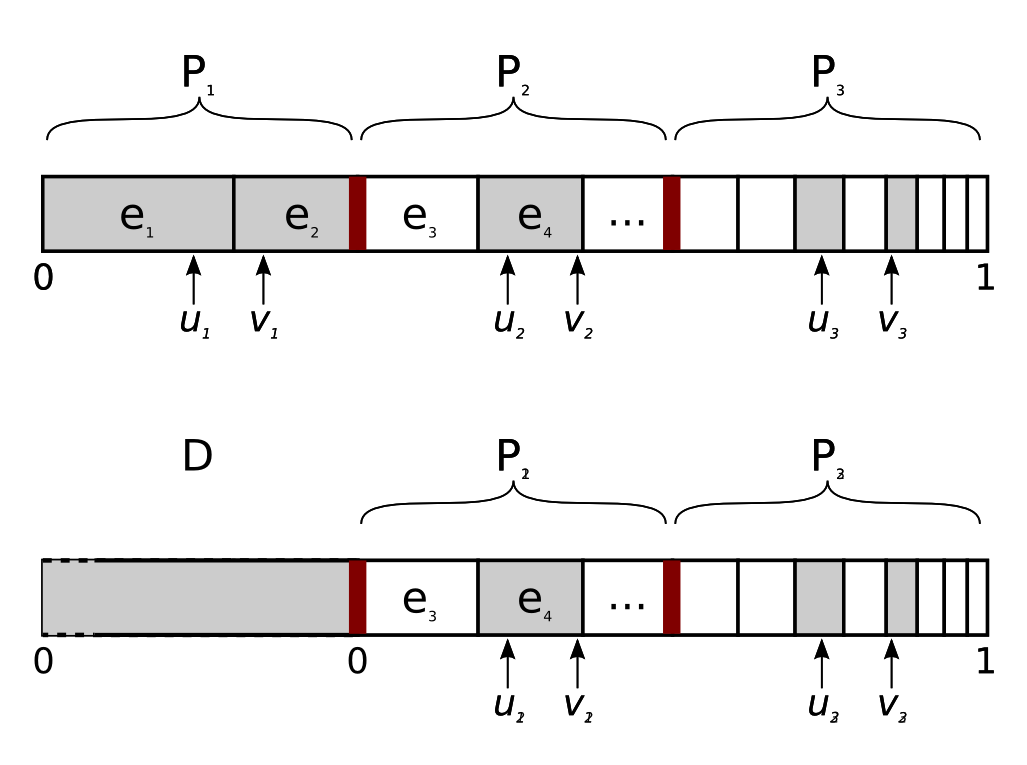
\includegraphics[width=0.9\columnwidth]{figures/pt2/move_to_deterministic}
		\caption{A REFAIRE NOTATION.............}
		\label{fig:move_to_deterministic}
		$E(I)$
	\end{center}
\end{figure}


\begin{figure}[h!]
	\begin{center}
		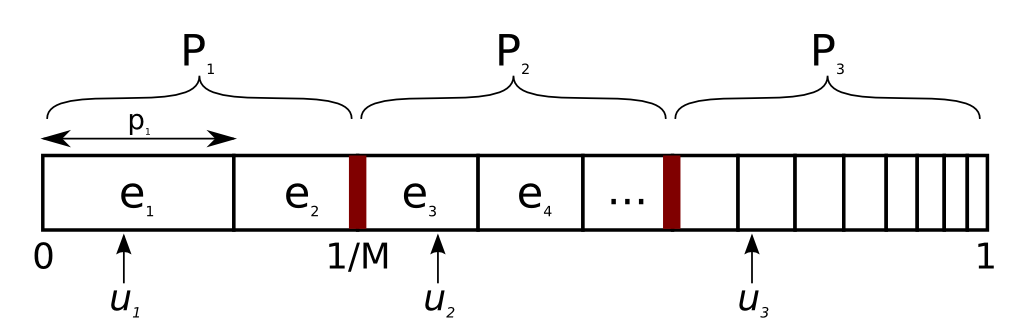
\includegraphics[width=0.9\columnwidth]{figures/pt2/comb}
		\caption{A REFAIRE NOTATION.............}
		\label{fig:comb}
		$E(I)$
	\end{center}
\end{figure}


\begin{figure}[h!]
	\begin{center}
		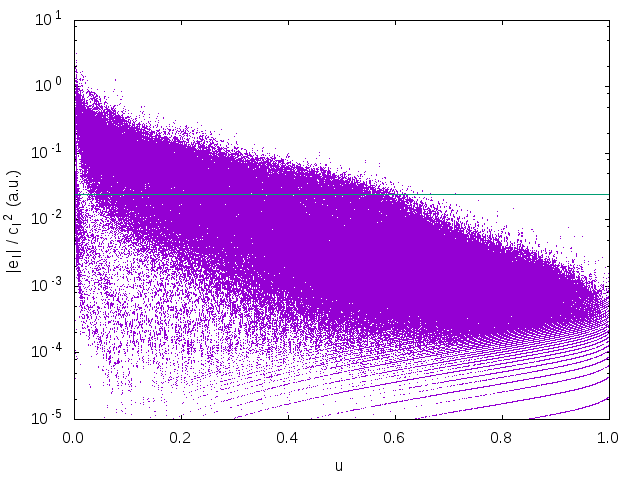
\includegraphics[width=0.9\columnwidth]{figures/pt2/eici2}
		\caption{A REFAIRE NOTATION.............}
		\label{fig:eici2}
		$E(I)$
	\end{center}
\end{figure}


\begin{figure}[h!]
	\begin{center}
		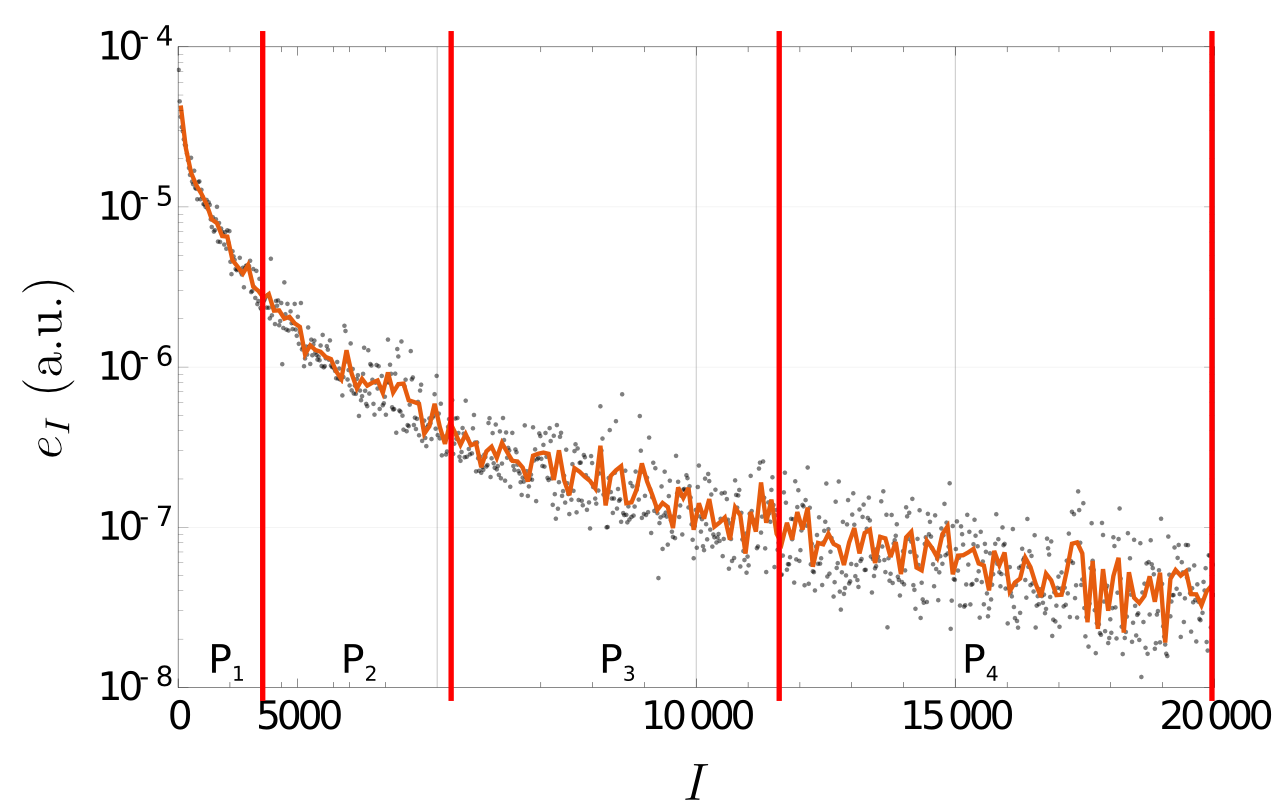
\includegraphics[width=0.9\columnwidth]{figures/pt2/P_i}
		\caption{A REFAIRE NOTATION.............}
		\label{fig:p_i}
		$E(I)$
	\end{center}
\end{figure}


\begin{figure}[h!]
	\begin{center}
		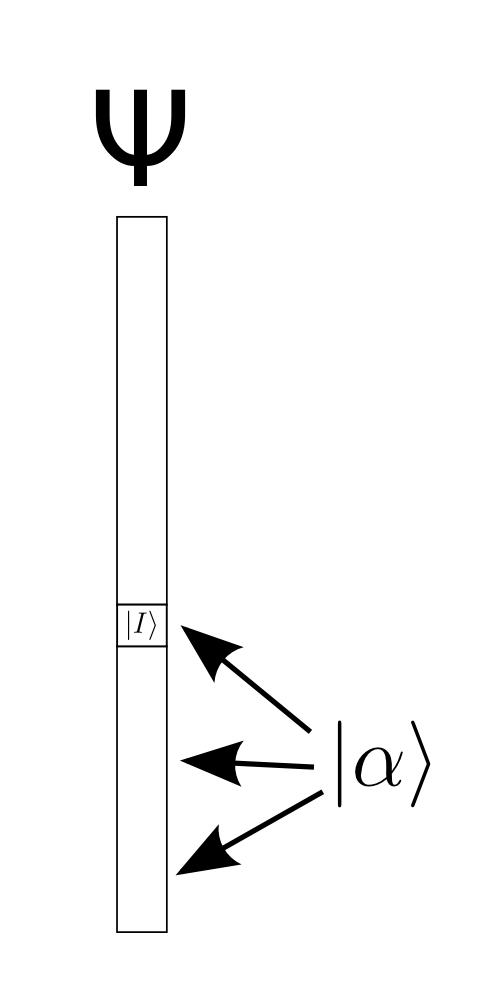
\includegraphics[width=0.2\columnwidth]{figures/pt2/a_con}
		\caption{A REFAIRE NOTATION.............}
		\label{fig:a_con}
		$\ket \alpha$ generated by increasing $\Psi_i$ connect to smaller and smaller norm of $\Psi$.
	\end{center}
\end{figure}

\begin{figure}[h!]
	\begin{center}
		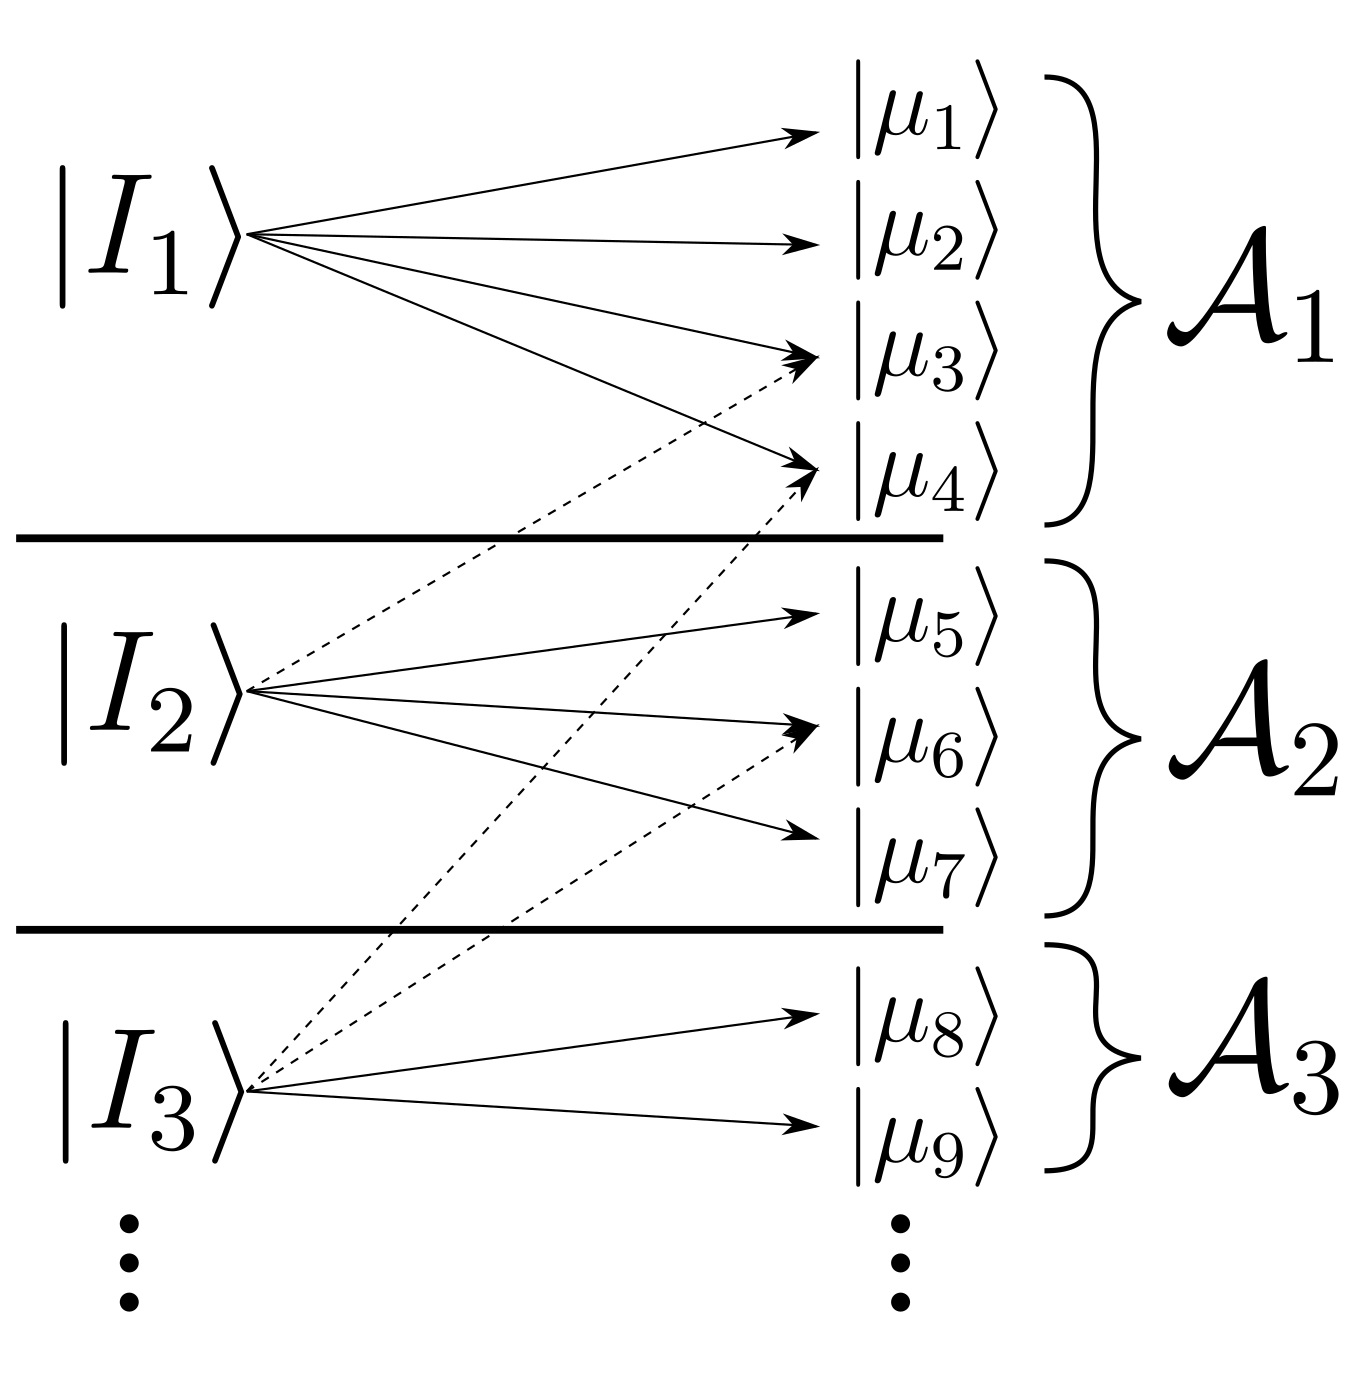
\includegraphics[width=0.5\columnwidth]{figures/pt2/mu_sample}
		\caption{}
		\label{fig:mu_sample}
		Construction of batches of $\ket \alpha$
	\end{center}
\end{figure}



\begin{figure}[h!]
	\label{comb_variables}
	\begin{center}
		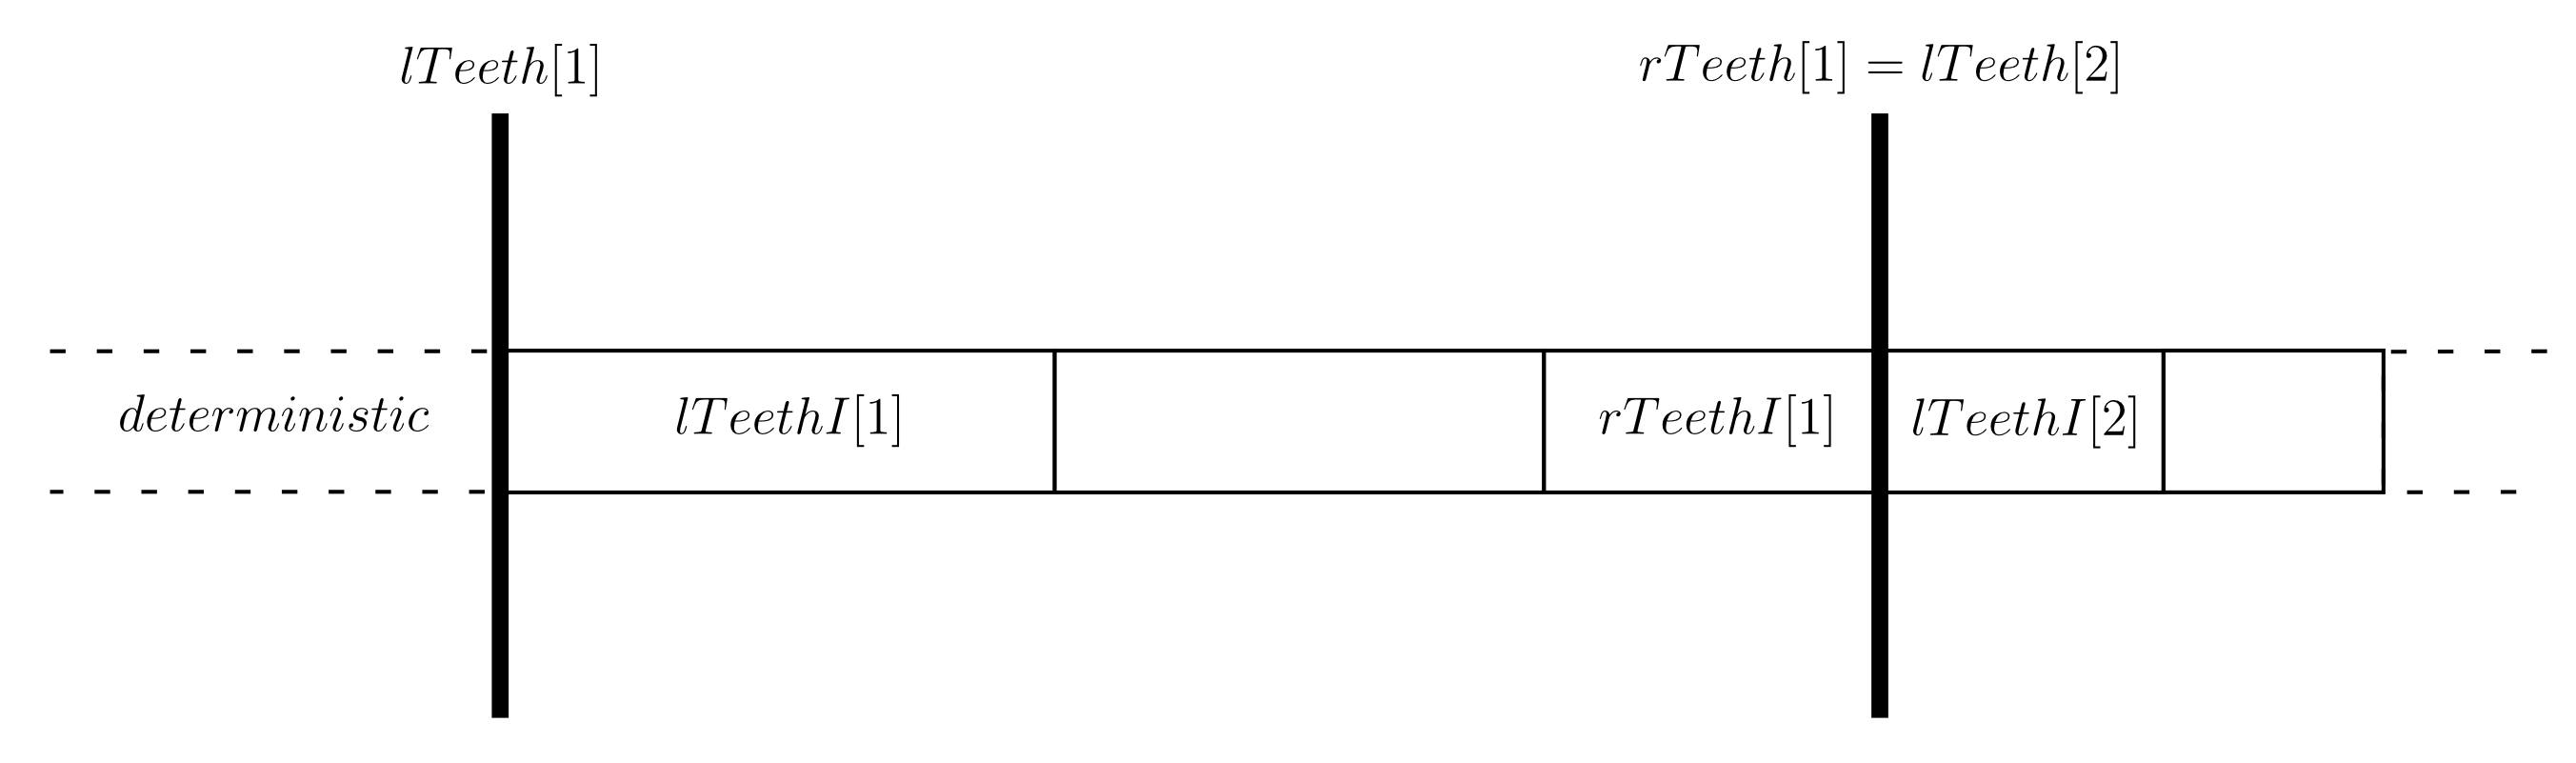
\includegraphics[width=1.00\columnwidth]{figures/pt2/teeth}
		\caption{comb}
		Variable names for the "comb" partition of $\Psi$. In boxes are shown indices, above are shown probabilities
		$$toothOfDet[i] = t ; i \in \big [ lTeethI[t],rTeethI[t] \big ]$$
		$$toothSize[t] = rTeeth[t] - lTeeth[t]$$
	\end{center}
\end{figure}

\begin{figure}[h!]
	\begin{center}
		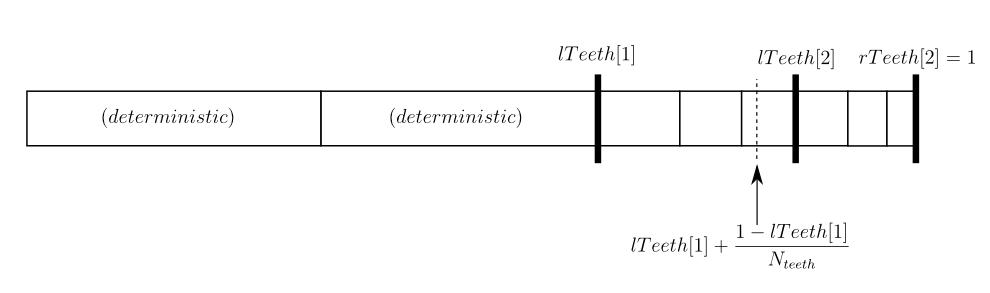
\includegraphics[width=1.00\columnwidth]{figures/pt2/teeths}
		\caption{\label{filtering}}
		Construction of teeth with $N_{teeth} = 2$ and 2 samples in the initial deterministic set.
	\end{center}
\end{figure}

\begin{figure}[h!]
	\begin{center}
		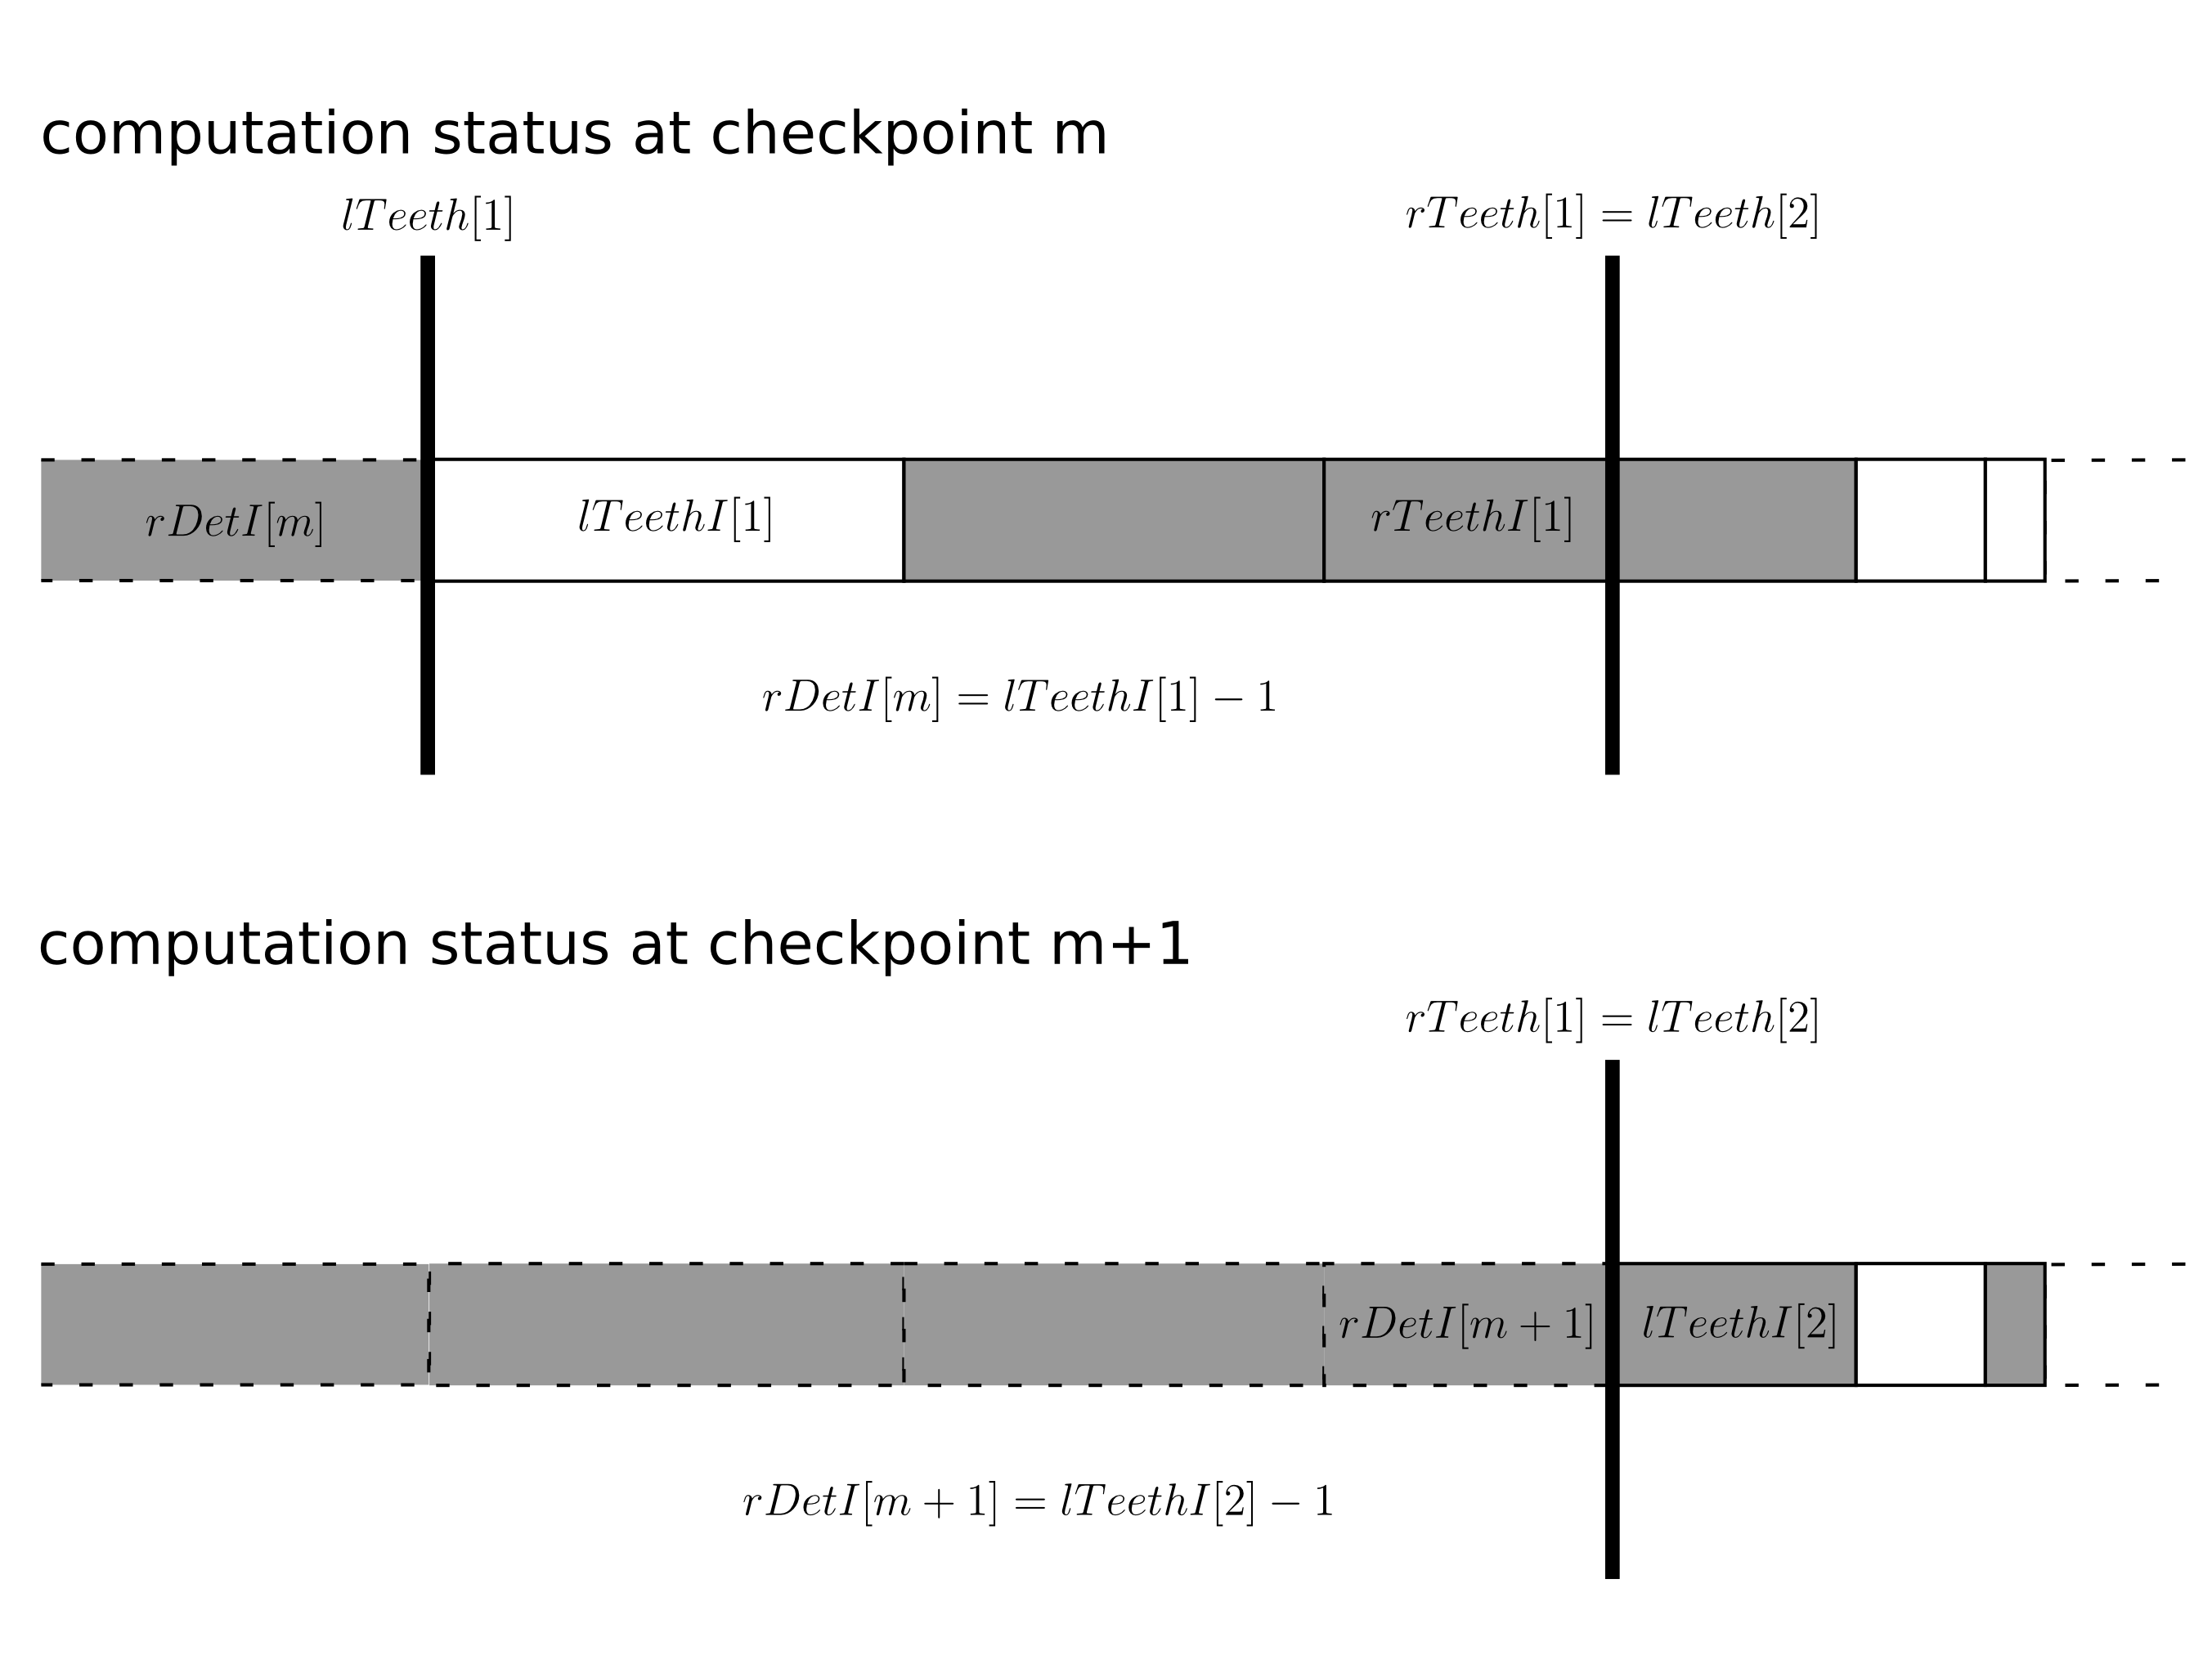
\includegraphics[width=1.00\columnwidth]{figures/matrix_dressing/deterministic_cp}
		\caption{\label{filtering}}
		$rDetI[m]$ gives the index of the last sample of the deterministic part at checkpoint $m$, or $0$ if there is no deterministic part.
		Greyed samples have been computed. Dotted samples are in the deterministic part. Sample $lTeethI[1]$ has been computed between checkpoints $m$ and $m+1$, resulting in tooth $1$ begin fully computed and thus moved into the deterministic part.
	\end{center}
\end{figure}

\end{document}
